\section{What we discussed last time}
\subsection{Prediction of pH using PU learning}
\begin{frame}{Performance of pH using PU learning }
\begin{columns}[T,onlytextwidth]		
	\begin{column}{0.5\textwidth}
		\begin{figure}
			\centering
			\includegraphics[width=1\linewidth]{../../msc-thesis-code/data/dataExploration/plots/train_0.25}
		\end{figure}
	\end{column}
	

	\begin{column}{0.5\textwidth}			
		\begin{figure}
			\centering
			\includegraphics[width=1\linewidth]{../../msc-thesis-code/data/dataExploration/plots/val_0.25}
		\end{figure}
	\end{column}		
	
\end{columns}	
\end{frame}


\section{What I did since then}
\begin{frame}{Model selection \& Label cleaning}
	\begin{columns}[T,onlytextwidth]		
		\begin{column}{0.5\textwidth}
			\begin{itemize}
				\item \small More thorough comparison of model
				\item \small test joinedTail, separateTails, RF and XGBoost
				\item XGBoost wins by far so focusing on that
			\end{itemize}
		\end{column}
			
			
			\begin{column}{0.5\textwidth}			
				\begin{itemize}
					\item \small Finetune large language model to improve parsing and handling of more obscure free text descriptions → not much better than parsing in the end (\textbf{on hold})
					\item \small Implement Condition Encoding using SMILES and Morgan fingerprints → worked to a degree using HDBSCAN majority of conditions can be clustered meaningfully, however 25\% were outliers (\textbf{in progress})
					\item \small implement sequence similarity based clustering
				\end{itemize}
			\end{column}		
			
		\end{columns}	
	\end{frame}


\begin{frame}{Sequence similarity based clustering for validation split}
	\begin{itemize}
		\item Sequences are clustered by similarity to group homologous proteins.
		\item Train/validation splits are performed at the cluster level.
		\item Clustering thresholds control homology between splits.
		\item Higher thresholds yield easier splits with similar sequences.
		\item Coarser clustering (e.g.\ 30\%) creates the hardest split with maximal dissimilarity.
	\end{itemize}
\end{frame}

\begin{frame}{Generalization Study}
	\begin{columns}[T,onlytextwidth]		
		\begin{column}{0.3\textwidth}
			\begin{itemize}
				\item \small Different levels tested 30\%, 40\%, 50\%,70\%,90,\%95\%,100\%
				\item \small Model loses generalization power extremely quickly 
				\item \small likely performs nearest neighbor in high dimensional embedding spacex
			\end{itemize}
		\end{column}
		
		
		\begin{column}{0.6\textwidth}			
			\begin{figure}
				\centering
				\includegraphics[width=1\linewidth]{../../msc-thesis-code/data/dataExploration/plots/cluster_similarity_performance}
			\end{figure}
		\end{column}		
		
	\end{columns}	
\end{frame}

\begin{frame}{Comparison 90 vs. 100 }
	\begin{columns}[T,onlytextwidth]		
		\begin{column}{0.5\textwidth}
			\begin{figure}
				\centering
				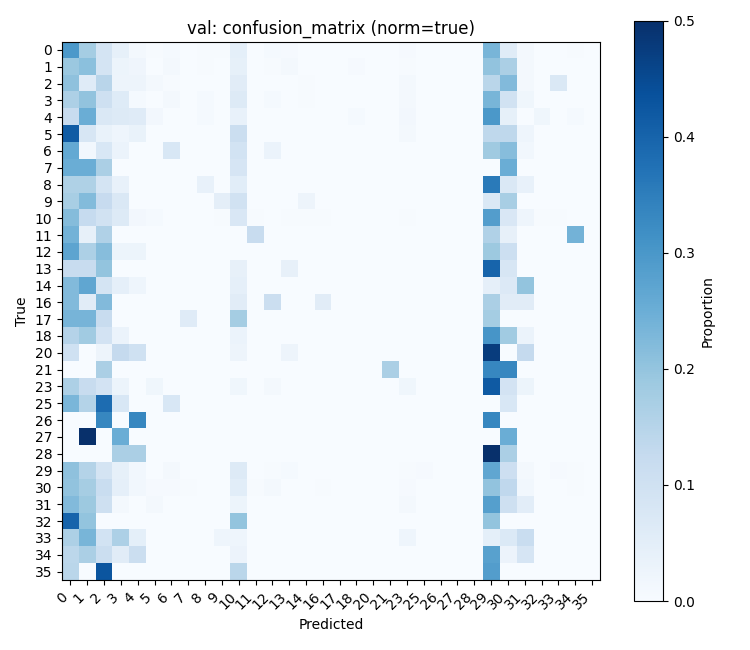
\includegraphics[width=1\linewidth]{media/seq_sim_90}
			\end{figure}
		\end{column}
		
		
		\begin{column}{0.5\textwidth}			
			\begin{figure}
				\centering
				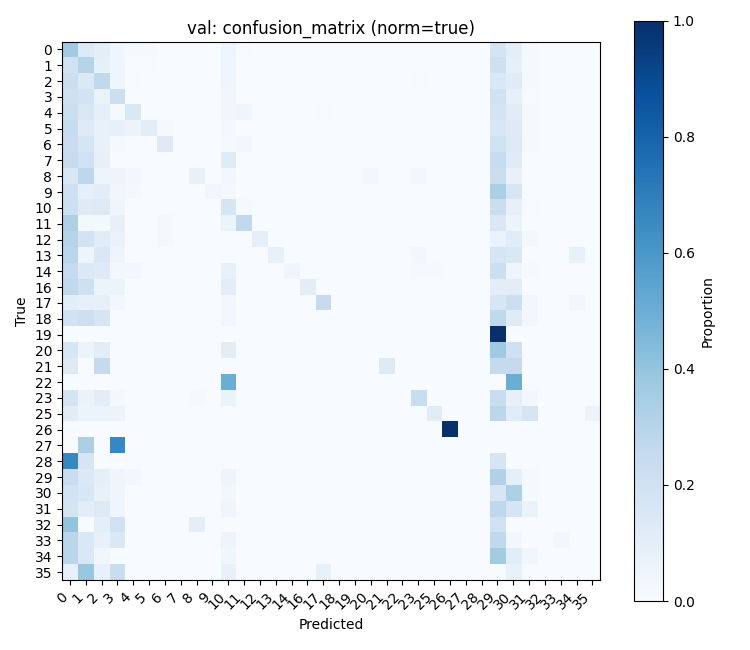
\includegraphics[width=1\linewidth]{media/seq_sim_100}
			\end{figure}
		\end{column}		
		
	\end{columns}	
\end{frame}

\begin{frame}{Questions \& Next steps}
	\begin{itemize}
	\item A lot of papers do not report sequence similarity based clustering for building a validation split. What would be a valid split? 
	\item Optimize PU learning for XGBoost
	\item Improve condition clustering and predict entire conditions instead of chemicals
	\end{itemize}	
\end{frame}

